\documentclass{beamer}
\usepackage[latin1]{inputenc}
\usepackage{listings}
\usetheme{Warsaw}

\title[Fault-tolerance on OdroidU3]{Embedded Systems Fault-tolerance}
\subtitle{A walkthrough from power-on to user-level application execution}

\author{Georgios Tziantzioulis}

\institute{Argonne National Laboratory}

\date{\today}

\begin{document}

\begin{frame}

  \titlepage

\end{frame}

\begin{frame}
  \frametitle{Outline}
  \tableofcontents[]
\end{frame}

\section{Introduction}

\subsection{Embedded Systems}
\begin{frame}{Embedded Systems}
  \begin{block}{Embedded Systems [Wikipedia]}
    are computer systems with a dedicated function within a larger mechanical or electrical system.
  \end{block}
\end{frame}


\subsection{Fault-tolerance}
\begin{frame}{Fault-tolerance}
  \begin{block}{Fault-tolerance, a system's property that: [Wikipedia]}
    \begin{itemize}[<+->]
    \item enables the system to continue operating properly in the event of a failure of some of its components.
    \item allows a proportional, to the failure's severity degree, operating quality decreases, as compared to a naively designed system in which even a small failure can cause total breakdown.
    \end{itemize}  
  \end{block}
\end{frame}

\subsection{The OdroidU3}
\begin{frame}{Odroid U3}
  \begin{columns}[C] % contents are top vertically aligned
    \begin{column}{5cm} % each column can also be its own environment
      \begin{itemize}
      \item 1.7GHz Quad-Core processor and 2GByte RAM
      \item 10/100Mbps Ethernet with RJ-45 LAN Jack
      \item 3 x High speed USB2.0 Host ports
      \item GPIO/UART/I2C ports
      \item Micro-SD slot, eMMC module connector
      \item 5V / 2A input
      \end{itemize}
    \end{column}
    \begin{column}{5cm} % alternative top-align that's better for graphics
      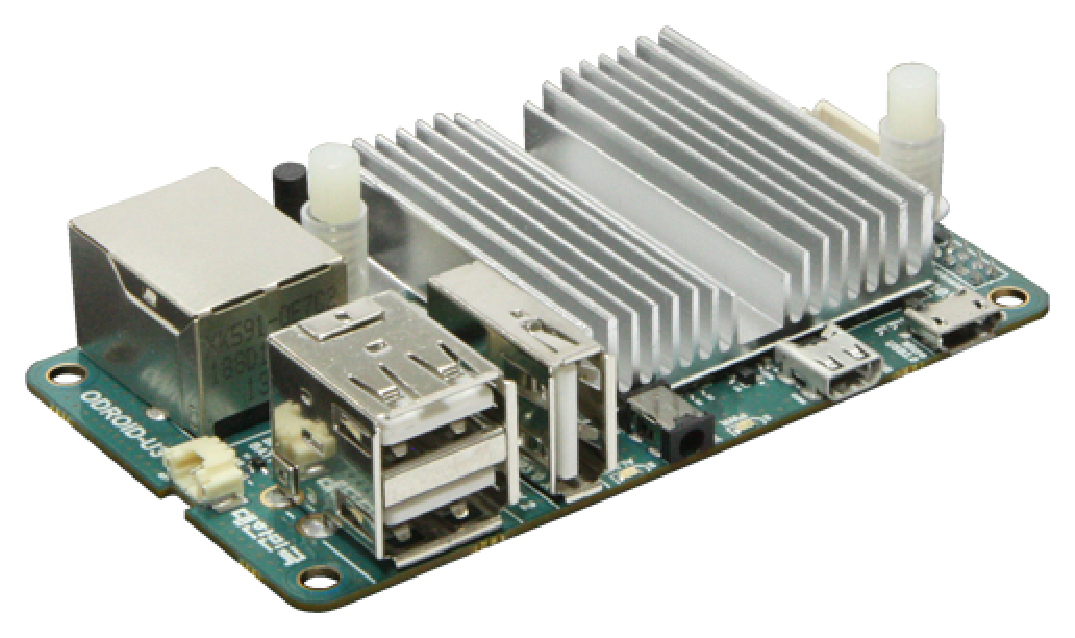
\includegraphics[width=5cm]{images/201312222305368236.eps}
    \end{column}
  \end{columns}
\end{frame}

\subsection{Motivation}
\begin{frame}{Motivation: Waggle Fault-tolerance}
  \begin{columns}[C] % contents are top vertically aligned
    \begin{column}{5cm} % each column can also be its own environment
      \begin{itemize}
      \item Deployed in an open environment (urban or rural)
      \item High cost of maintainance due to volume of devices
      \item Requirement for high availability (node part)
      \end{itemize}
    \end{column}
    \begin{column}{5cm} % alternative top-align that's better for graphics
      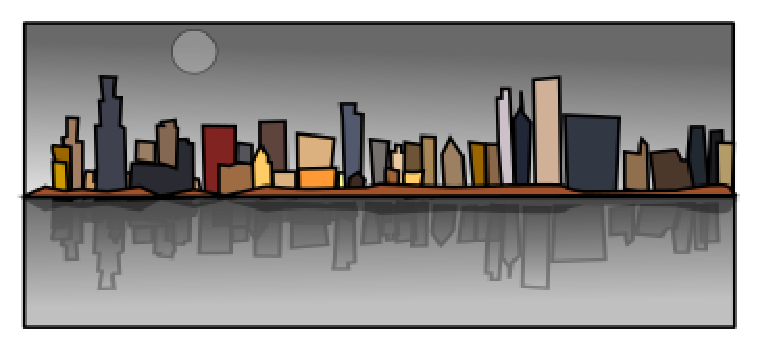
\includegraphics[width=5cm]{images/chicago.eps}

      
\includegraphics[width=5cm]{images/montagne.eps}
    \end{column}
  \end{columns}
\end{frame}

\section{High-level Picture}

\begin{frame}{Odroid U3: From power-on to user-level applications}
\frametitle{The High-level Picture}
  \begin{columns}[C] % contents are top vertically aligned
    \begin{column}{5cm} % each column can also be its own environment
      \begin{enumerate}
      \item Power-on
      \item Bootloader
      \item Operating System Kernel
      \item Initialization
      \item User-level Applications
      \end{enumerate}
    \end{column}
    \begin{column}{5cm} % alternative top-align that's better for graphics
      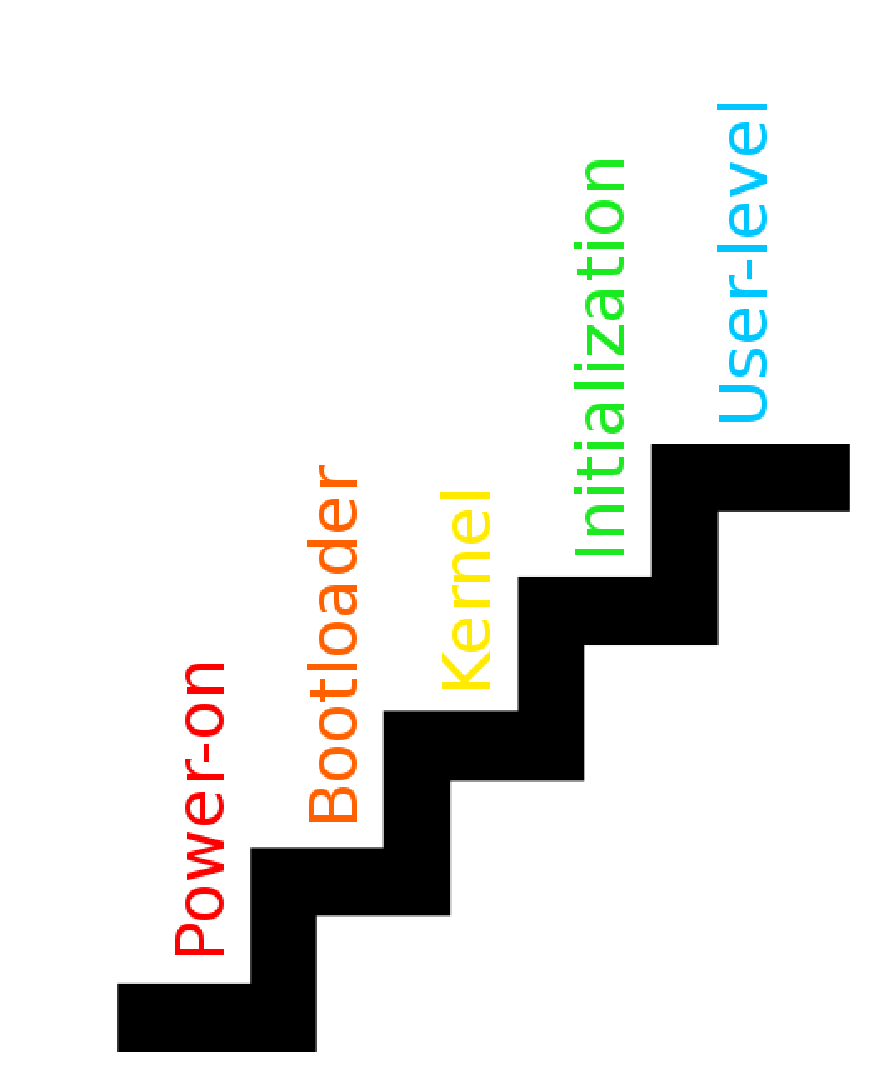
\includegraphics[width=5cm]{images/aiga_stairs_2.eps}
    \end{column}
  \end{columns}
\end{frame}

\section{In details}

\subsection{Power-on}
\begin{frame}
\frametitle{Power-on}
  \begin{columns}[C]
    \begin{column}{5cm}
      \begin{block}{Power-on}
        \begin{itemize}
        \item Hardware procedure (Finite-state machine)
        \item Vendor/device specific
        \end{itemize}  
      \end{block}
    \end{column}
    \uncover<2->{
      \begin{column}{5cm}
        \begin{alertblock}{Fault-tolerance}
          \begin{itemize}[<+->]
          \item Zero flexibility due to closed design
          \end{itemize}  
        \end{alertblock}
      \end{column}
    }
  \end{columns}
\end{frame}

\subsection{Bootloader}
\begin{frame}
\frametitle{Bootloader}
  \begin{columns}[C] % contents are top vertically aligned
    \only<1-2>{
      \begin{column}{5cm} % each column can also be its own environment
        \begin{block}{Bootloader}
          \begin{itemize}
          \item Platform/architecture specific (ARM)
          \item Power-on self-test
          \item Initialize devices needed to launch the operating system
          \item Potentially multiple stages
          \end{itemize}
        \end{block}
      \end{column}
    }
    \only<2-3>{
      \begin{column}{5cm} % each column can also be its own environment
        \begin{block}{Odroid U3 bootloader}
          \begin{itemize}
          \item 4 stages
            \begin{enumerate}
            \item iROM (processor specific)
            \item BL1 (Samsung)
            \item BL2 (Das U-Boot SPL)
            \item Das U-Boot
            \end{enumerate}
          \item BL1 and BL2 signed by Samsung
          \end{itemize}
        \end{block}
      \end{column}
    }
    \only<3>{
      \begin{column}{5cm} % alternative top-align that's better for graphics
        \begin{alertblock}{Fault-tolerance (Das U-Boot)}
          \begin{enumerate}
          \item Power-on self-test (limited)
          \item Kernel image verification (uImage, FIT)
          \item Conditional booting (boot script)
          \item Support for journaling file system (ext4)
          \end{enumerate}
        \end{alertblock}
      \end{column}
    }
    %% \only<4->{
    %%   \begin{column}{5cm}
    %%     \lstinputlisting[basicstyle=\tiny]{code/boot.txt}
    %%   \end{column}
    %% }
  \end{columns}
\end{frame}

\subsection{Operating System Kernel}
\begin{frame}
\frametitle{Kernel}
  \begin{columns}[C] % contents are top vertically aligned
    \only<1>{
      \begin{column}{5cm} % each column can also be its own environment
        \begin{block}{Linux is: [Wikipedia]}
          a Unix-like and (mostly) POSIX-compliant computer operating system assembled under the model of free and open source software development and distribution
        \end{block}
      \end{column}
    }
    \only<2->{
      \begin{column}{5cm}
        \begin{block}{Linux}
          \begin{itemize}
          \item Open Source
          \item Support for multiple architectures
          \item Support for wide range of devices
          \item Open Source
          \end{itemize}
        \end{block}
      \end{column}
      \begin{column}{5cm} % alternative top-align that's better for graphics
        \begin{alertblock}{Fault-tolerance}
          \begin{enumerate}
          \item Force restart after crash (sysctl.conf)
          \item Clean after module crash (auto)
          \item Minimum number of modules
          \end{enumerate}
        \end{alertblock}
      \end{column}
    }
  \end{columns}
\end{frame}

\subsection{Initialization}
\begin{frame}
\frametitle{Initialization}
  \frametitle{Initialize services}
  \begin{columns}[C] % contents are top vertically aligned
    \begin{column}{5cm} % each column can also be its own environment
      \begin{enumerate}
      \item (initramfs)
      \item upstart
      \item monit
      \end{enumerate}
    \end{column}
    \only<2>{
      \begin{column}{5cm} % alternative top-align that's better for graphics
        \begin{block}{initramfs is: [Wikipedia]}
          an archive of a minimal file system loaded and operated into memory during the Linux startup process.
        \end{block}
        \begin{alertblock}{Fault-tolerance}
          \begin{enumerate}
          \item File System check
          \item Full use of cpu sets framework (through init)
          \end{enumerate}
        \end{alertblock}
      \end{column}
    }
    \only<3>{
      \begin{column}{5cm} % alternative top-align that's better for graphics
        \begin{block}{Upstart is: [Wikipedia]}
          an event-based replacement for the traditional init daemon
        \end{block}
        \begin{alertblock}{Fault-tolerance}
          \begin{enumerate}
          \item Respawn sevices
          \item Logging
          \item Initialize cpu sets
          \end{enumerate}  
        \end{alertblock}
      \end{column}
    }
  \only<4>{
    \begin{column}{5cm}
      \begin{block}{Monit is: [Wikipedia]}
        a free, open source process supervision tool for Unix and Linux
      \end{block}
      \begin{alertblock}{Fault-tolerance}
        \begin{enumerate}
        \item Services respawn
        \item Service monitoring
        \item Rule enforcement (checksum, permissions, do X after N crashes)
        \item Event notification
        \end{enumerate}
      \end{alertblock}
    \end{column}
  }
\end{columns}
\end{frame}

\subsection{User-level Applications}
\begin{frame}
\frametitle{User-level Applications}
\begin{center}
  Nothing yet
\end{center}
\end{frame}

\section{Demo}
\begin{frame}
  \begin{columns}[C]
    \column{5cm}
    \begin{center}
      Demo
    \end{center}
    \includegraphics[width=5cm]{images/liftarn_Smashed_TV.eps}  
  \end{columns}
  %% \btVFill
  \vskip0pt plus 1filll
  \tiny{For all images used in this presentation credit @ openclipart.org}
\end{frame}

\end{document}
